% Copyright (c) 2026 CorrectBrain
% SPDX-License-Identifier: MIT

\PassOptionsToPackage{dvipsnames,svgnames,x11names}{xcolor}
\documentclass[tikz,border=8pt]{standalone}
\usetikzlibrary{arrows.meta,positioning,calc,shapes,shadows,decorations.pathmorphing,shapes.geometric,backgrounds,decorations.markings,decorations.pathreplacing,decorations.text,fit,shapes.misc,shapes.arrows,matrix,bending,3d,chains,intersections,shapes.symbols,svg.path,shapes.multipart,snakes,shapes.callouts,angles,quotes}
\providecolor{gold}{RGB}{212,175,55}
\providecolor{silver}{RGB}{192,192,192}
\providecolor{bronze}{RGB}{205,127,50}
\providecolor{darkblue}{RGB}{0,0,139}
\providecolor{lightblue}{RGB}{173,216,230}
\providecolor{darkgreen}{RGB}{0,100,0}
\providecolor{lightgreen}{RGB}{144,238,144}
\providecolor{darkred}{RGB}{139,0,0}
\providecolor{navy}{RGB}{0,0,128}
\providecolor{skyblue}{RGB}{135,206,235}
\providecolor{beige}{RGB}{245,245,220}
\providecolor{cream}{RGB}{255,253,208}
\usepackage{amsmath}
\usepackage{amssymb}
\usepackage{fontawesome5}
\usetikzlibrary{fadings,shadows.blur,patterns,patterns.meta}

\providecolor{gold}{RGB}{212,175,55}
\providecolor{silver}{RGB}{192,192,192}
\providecolor{bronze}{RGB}{205,127,50}
\providecolor{darkblue}{RGB}{0,0,139}
\providecolor{lightblue}{RGB}{173,216,230}
\providecolor{darkgreen}{RGB}{0,100,0}
\providecolor{lightgreen}{RGB}{144,238,144}
\providecolor{darkred}{RGB}{139,0,0}
\providecolor{navy}{RGB}{0,0,128}
\providecolor{skyblue}{RGB}{135,206,235}
\providecolor{beige}{RGB}{245,245,220}
\providecolor{cream}{RGB}{255,253,208}
\usepackage{amsmath}
\usepackage{amssymb}
\usepackage{fontawesome5}


\providecolor{gold}{RGB}{212,175,55}
\providecolor{silver}{RGB}{192,192,192}
\providecolor{bronze}{RGB}{205,127,50}
\providecolor{darkblue}{RGB}{0,0,139}
\providecolor{lightblue}{RGB}{173,216,230}
\providecolor{darkgreen}{RGB}{0,100,0}
\providecolor{lightgreen}{RGB}{144,238,144}
\providecolor{darkred}{RGB}{139,0,0}
\providecolor{navy}{RGB}{0,0,128}
\providecolor{skyblue}{RGB}{135,206,235}
\providecolor{beige}{RGB}{245,245,220}
\providecolor{cream}{RGB}{255,253,208}
\usepackage{amsmath}
\usepackage{amssymb}
\usepackage{fontawesome5}
\usepackage{xcolor}

% --- SYNTAX HIGHLIGHTING COLORS (Dracula Theme) ---
\definecolor{codebg}{RGB}{40, 42, 54}
\definecolor{codeheader}{RGB}{30, 32, 42}
\definecolor{codetext}{RGB}{248, 248, 242}
\definecolor{keyword}{RGB}{139, 233, 253}
\definecolor{string}{RGB}{241, 250, 140}
\definecolor{variable}{RGB}{255, 121, 198}
\definecolor{property}{RGB}{80, 250, 123}
\definecolor{value}{RGB}{189, 147, 249}
\definecolor{selector}{RGB}{255, 184, 108}
\definecolor{comment}{RGB}{98, 114, 164}

% --- WINDOW CONTROL BUTTON COLORS ---
\definecolor{btnclose}{RGB}{255, 95, 86}
\definecolor{btnmin}{RGB}{255, 189, 46}
\definecolor{btnmax}{RGB}{39, 201, 63}

% --- GEOMETRY COLORS ---
\definecolor{brandprimary}{RGB}{255, 64, 129} % Pink (#FF4081)
\definecolor{brandhover}{RGB}{0, 229, 255}    % Cyan (#00E5FF)

\begin{document}
\begin{tikzpicture}

% --- GLOBAL CANVAS BACKGROUND ---
\fill[white] (-0.5, -1.0) rectangle (24.0, 16.5);

% --- TITLE SECTION ---
\node[font=\Huge\bfseries, text=black!85, align=center] at (11.75, 15.5) {Deep Topological Targeting \& CSS Custom Variables};
\node[font=\Large, text=black!60, align=center] at (11.75, 14.7) {Mapping runtime variables and pseudo-class states to SVG vector geometry};


% ============================================================================
% 1. CODE EDITOR PANE (LEFT)
% ============================================================================
% Window container
\draw[fill=codebg, draw=black!40, thick, rounded corners=8pt, blur shadow={shadow opacity=35, shadow blur steps=5, shadow xshift=2pt, shadow yshift=-3pt}]
  (0.5, 5.5) rectangle (9.5, 13.5);

% Title bar with macOS style controls
\path[fill=codeheader, rounded corners=8pt] (0.5, 12.7) rectangle (9.5, 13.5);
\fill[codeheader] (0.5, 12.7) rectangle (9.5, 13.0); % square off bottom of header
\draw[black!60, thick] (0.5, 12.7) -- (9.5, 12.7);

% Window action buttons
\fill[btnclose] (1.0, 13.1) circle (0.13cm);
\fill[btnmin]   (1.4, 13.1) circle (0.13cm);
\fill[btnmax]   (1.8, 13.1) circle (0.13cm);

% Editor title
\node[font=\large\bfseries, text=codetext] at (5.0, 13.1) {\faFileCode\ styles.css};

% Code Body with exact line alignment
\node[anchor=north west, font=\ttfamily\small, text=codetext, align=left, inner sep=0pt] at (0.8, 12.5) {
\color{selector}:root \color{codetext}\{ \\
\quad \color{variable}--brand-primary\color{codetext}: \color{value}\#FF4081\color{codetext}; \\
\quad \color{variable}--brand-hover\color{codetext}: \color{value}\#00E5FF\color{codetext}; \\
\color{codetext}\} \\[5pt]
\color{comment}/* 1. Structural targeting via inheritance */ \\
\color{selector}\#data-node .outer-ring, \#data-node .core \color{codetext}\{ \\
\quad \color{property}fill\color{codetext}: \color{keyword}var\color{codetext}(\color{variable}--brand-primary\color{codetext}); \\
\quad \color{property}transition\color{codetext}: \color{property}fill \color{value}0.3s ease\color{codetext}; \\
\color{codetext}\} \\[5pt]
\color{comment}/* 2. Complex DOM Hit-Testing \& State Mapping */ \\
\color{selector}\#data-node:hover .inner-sector \color{codetext}\{ \\
\quad \color{property}fill\color{codetext}: \color{keyword}var\color{codetext}(\color{variable}--brand-hover\color{codetext}); \\
\quad \color{property}transform\color{codetext}: \color{value}rotate\color{codetext}(\color{value}90deg\color{codetext}); \\
\quad \color{property}transform-origin\color{codetext}: \color{value}center\color{codetext}; \\
\color{codetext}\}
};

% Port nodes on code window border
\fill[brandprimary] (9.5, 9.5) circle (2.5pt);
\fill[brandhover]   (9.5, 7.0) circle (2.5pt);


% ============================================================================
% 2. BROWSER RENDER VIEWPORT (RIGHT)
% ============================================================================
% Viewport container
\draw[fill=blue!1!white, draw=black!25, thick, rounded corners=8pt, blur shadow={shadow opacity=20, shadow blur steps=5, shadow xshift=2pt, shadow yshift=-3pt}]
  (11.0, 5.5) rectangle (23.0, 13.5);

% Viewport Header Bar
\path[fill=gray!12, rounded corners=8pt] (11.0, 12.7) rectangle (23.0, 13.5);
\fill[gray!12] (11.0, 12.7) rectangle (23.0, 13.0);
\draw[black!15, thick] (11.0, 12.7) -- (23.0, 12.7);

\node[font=\large\bfseries, text=black!75] at (17.0, 13.1) {\faDrawPolygon\ Browser Render (SVG DOM)};

% Monospace DOM Tags in Viewport Left Side (Segregated from Grid)
\node[anchor=north west, font=\ttfamily\scriptsize, text=black!35, align=left, inner sep=0pt, text width=4.5cm] at (11.3, 12.4) {
<svg id="stage" \\
\quad viewBox="0 0 500 500"> \\
\quad <g id="data-node"> \\
\qquad <path class="outer-ring" ... /> \\
\qquad <path class="inner-sector" ... /> \\
\qquad <circle class="core" cx="250" cy="250" r="50" /> \\
\quad </g> \\
</svg>
};

% 100px = 1.0 unit Grid (500x500 viewBox)
\draw[step=1.0, black!6, thin] (17.0, 7.0) grid (22.0, 12.0);

% Origin (0,0) and Inverted SVG Coordinate Axes (Downwards Y-axis)
\draw[-Stealth=3mm, black!45, thick] (17.0, 12.0) -- (22.3, 12.0) node[anchor=west, font=\scriptsize\bfseries\sffamily] {x};
\draw[-Stealth=3mm, black!45, thick] (17.0, 12.0) -- (17.0, 6.7)  node[anchor=north, font=\scriptsize\bfseries\sffamily] {y};

% X-axis Scale Markers (top)
\node[font=\tiny\ttfamily, text=black!45, anchor=south] at (17.0, 12.1) {(0,0)};
\node[font=\tiny\ttfamily, text=black!45, anchor=south] at (18.0, 12.1) {100};
\node[font=\tiny\ttfamily, text=black!45, anchor=south] at (19.0, 12.1) {200};
\node[font=\tiny\ttfamily, text=black!45, anchor=south] at (20.0, 12.1) {300};
\node[font=\tiny\ttfamily, text=black!45, anchor=south] at (21.0, 12.1) {400};
\node[font=\tiny\ttfamily, text=black!45, anchor=south] at (22.0, 12.1) {500};

% Y-axis Scale Markers (placed on the LEFT of Y-axis line to avoid text overlap)
\node[font=\tiny\ttfamily, text=black!45, anchor=east] at (16.8, 11.0) {100};
\node[font=\tiny\ttfamily, text=black!45, anchor=east] at (16.8, 10.0) {200};
\node[font=\tiny\ttfamily, text=black!45, anchor=east] at (16.8, 9.0)  {300};
\node[font=\tiny\ttfamily, text=black!45, anchor=east] at (16.8, 8.0)  {400};
\node[font=\tiny\ttfamily, text=black!45, anchor=east] at (16.8, 7.0)  {500};


% ============================================================================
% 3. THE GEOMETRIC NODE (Mathematically locked at cx=250, cy=250 -> (19.5, 9.5))
% ============================================================================
\coordinate (NodeCenter) at (19.5, 9.5);

% Neon Ambient Glows behind Geometry
\fill[brandprimary!12, opacity=0.6] (NodeCenter) circle (2.45cm);
\fill[brandprimary!20, opacity=0.5] (NodeCenter) circle (2.30cm);

% State Indicator: Hover Ring
\draw[thick, brandhover!60, dashed] (NodeCenter) circle (2.55cm);

% 1. Outer Ring (Targeted by --brand-primary, radius = 2.0cm, line width = 2.8pt)
\draw[fill=codebg, draw=brandprimary, line width=2.8pt] (NodeCenter) circle (2.0cm);
\draw[draw=brandprimary!35, line width=5.5pt, opacity=0.4] (NodeCenter) circle (2.0cm);

% 2. Kinetic Rotational State Indicators (Hover state, radius = 2.3cm)
\draw[-Stealth=3mm, line width=1.6pt, brandhover]
  (NodeCenter) ++(45:2.3cm) arc (45:135:2.3cm);
\draw[-Stealth=3mm, line width=1.6pt, brandhover]
  (NodeCenter) ++(225:2.3cm) arc (225:315:2.3cm);
\draw[dashed, brandhover!40, line width=1.2pt]
  (NodeCenter) ++(-45:2.3cm) arc (-45:45:2.3cm);
\draw[dashed, brandhover!40, line width=1.2pt]
  (NodeCenter) ++(135:2.3cm) arc (135:225:2.3cm);

% 3. Inner Sectors (Targeted by hover, radius = 1.5cm)
\fill[brandhover!30, opacity=0.7] (NodeCenter) -- +(45:1.55cm) arc (45:135:1.55cm) -- cycle;
\fill[brandhover!30, opacity=0.7] (NodeCenter) -- +(225:1.55cm) arc (225:315:1.55cm) -- cycle;
\fill[brandhover] (NodeCenter) -- +(45:1.5cm) arc (45:135:1.5cm) -- cycle;
\fill[brandhover] (NodeCenter) -- +(225:1.5cm) arc (225:315:1.5cm) -- cycle;

% 4. Core Structure (Targeted by --brand-primary, r=50 -> 0.5cm)
\fill[brandprimary!30, opacity=0.6] (NodeCenter) circle (0.65cm);
\fill[brandprimary] (NodeCenter) circle (0.5cm);
\fill[white!50, opacity=0.6] ([shift={(-0.12, 0.12)}]NodeCenter) circle (0.12cm); % glossy light reflection


% ============================================================================
% 4. SHIELDED LABELS & BADGES (Zero Overlaps)
% ============================================================================
% path.outer-ring Label
\node[fill=white, draw=brandprimary!60, thick, rounded corners=3pt, inner sep=2.5pt, font=\scriptsize\ttfamily\bfseries, text=black!90, blur shadow={shadow opacity=15}] (OuterRingLabel)
  at (17.0, 4.8) {path.outer-ring};
\draw[draw=brandprimary!70, line width=1pt] (17.0, 5.2) -- (18.0, 8.0);

% circle.core Label
\node[fill=white, draw=brandprimary!60, thick, rounded corners=3pt, inner sep=2.5pt, font=\scriptsize\ttfamily\bfseries, text=black!90, blur shadow={shadow opacity=15}] (CoreLabel)
  at (19.5, 4.8) {circle.core};
\draw[draw=brandprimary!70, line width=1pt] (19.5, 5.2) -- (19.5, 9.0);

% path.inner-sector Label
\node[fill=white, draw=brandhover!60, thick, rounded corners=3pt, inner sep=2.5pt, font=\scriptsize\ttfamily\bfseries, text=black!90, blur shadow={shadow opacity=15}] (InnerSectorLabel)
  at (22.0, 4.8) {path.inner-sector};
\draw[draw=brandhover!70, line width=1pt] (22.0, 5.2) -- (20.5, 8.6);

% :hover state Tag
\node[fill=white, draw=brandhover, thick, rounded corners=4pt, inner sep=3pt, font=\small\bfseries, text=brandhover!80!black, blur shadow={shadow opacity=20}]
  at (21.8, 12.2) {\faMousePointer\ :hover state};
\draw[-Stealth=2mm, brandhover, thick, dashed] (21.8, 12.0) -- (21.3, 11.4);


% ============================================================================
% 5. ORTHOGONAL DATA PIPELINES (Routed through Highway Gap Y=3.5 to Y=5.5)
% ============================================================================
% Pink Pipeline (--brand-primary)
\draw[line width=1.8pt, brandprimary, rounded corners=6pt]
  (9.5, 9.5) -- (10.6, 9.5) -- (10.6, 4.2) -- (19.5, 4.2);

% Pink Pipeline Branch 1 -> path.outer-ring
\draw[-Stealth=3mm, line width=1.8pt, brandprimary, rounded corners=6pt]
  (17.0, 4.2) -- (OuterRingLabel.south);

% Pink Pipeline Branch 2 -> circle.core
\draw[-Stealth=3mm, line width=1.8pt, brandprimary, rounded corners=6pt]
  (19.5, 4.2) -- (CoreLabel.south);

\fill[brandprimary] (17.0, 4.2) circle (2.5pt);

% Cyan Pipeline (--brand-hover) -> path.inner-sector
\draw[-Stealth=3mm, line width=1.8pt, brandhover, rounded corners=6pt]
  (9.5, 7.0) -- (10.2, 7.0) -- (10.2, 3.8) -- (22.0, 3.8) -- (InnerSectorLabel.south);


% ============================================================================
% 6. BOTTOM EXPLANATION PANEL
% ============================================================================
\draw[fill=white, draw=black!20, thick, rounded corners=8pt, blur shadow={shadow opacity=20, shadow blur steps=5, shadow xshift=2pt, shadow yshift=-3pt}]
  (0.5, -0.5) rectangle (23.0, 3.5);

\node[anchor=north west, text width=21.0cm, inner sep=0pt] at (1.0, 3.0) {
    {\bfseries\Large Contextual Inheritance \& Geometric Statefulness}\\[6pt]
    By defining variables (\texttt{--brand-primary}) at the \texttt{:root}, the browser constructs a tunnel directly into the SVG topology. When the user switches to Dark Mode, updating the CSS variable recalculates the matrix and repaints the vector without HTTP requests. \\
    \vspace{4pt}
    Furthermore, because the DOM handles hit-testing, a \texttt{:hover} event on the parent \texttt{<svg>} allows precise CSS selectors to reach down and mutate specific descendant paths (e.g., rotating the cyan inner sectors) while leaving the rest of the geometric matrix intact.
};

\end{tikzpicture}
\end{document}
